\section{eplusout.wrl}\label{eplusout.wrl}

The VRML output report file is formatted according to the ``Virtual Reality Modeling Language'' standard rules for representing building type surfaces. The file can be used in several inexpensive, shareware or freeware viewers. There are a variety of stand alone and viewers integrated within browsers. A good list of viewers can be found at:

\url{http://cic.nist.gov/vrml/vbdetect.html}

This site detects what, if any, VRML plugin is installed in your browser as well as gives a list of active ones with links to their sites.

This file is generated when the following line is included in the IDF.

\textbf{Output:Surfaces:Drawing, VRML;}

In addition, like the DXF output, you can ask it to triangulate (algorithm within EnergyPlus) surfaces with \textgreater{}4 sides:

\textbf{Output:Surfaces:Drawing, VRML, Triangulate 3dface;}

Most viewers will illustrate a solid model by default:

\begin{figure}[hbtp] % fig 10
\centering
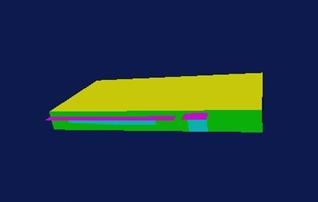
\includegraphics[width=0.9\textwidth, height=0.9\textheight, keepaspectratio=true]{media/image025.jpg}
\caption{VRML output - solid model \protect \label{fig:vrml-output-solid-model}}
\end{figure}

With some/many viewers, you can also see a wireframe model; some will even fill this model. Also, viewers can triangulate any surface that isn't labeled as ``convex'' by the software writing the file (i.e.~EnergyPlus). However, this triangulation may not be correct so you may wish to do it from within EnergyPlus as illustrated above.

A wireframe model of the same building as above is:

\begin{figure}[hbtp] % fig 11
\centering
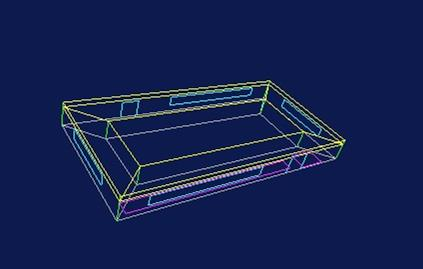
\includegraphics[width=0.9\textwidth, height=0.9\textheight, keepaspectratio=true]{media/image026.jpg}
\caption{VRML output - wireframe model \protect \label{fig:vrml-output-wireframe-model}}
\end{figure}

The actual file produced is a text file. EnergyPlus adds some comments, such as the list of zone names and surface names before each coordinate specification. The line/solid colors are set as Floor, Wall, etc. so the file is somewhat readable.

\begin{lstlisting}
#VRML V2.0 utf8
WorldInfo {
   title "Building - Building"
   info ["EnergyPlus Program Version EnergyPlus <version>, 9/14/2006 1:31 PM"]
}
# Zone Names
# Zone = 1:PLENUM-1
# Zone = 2:SPACE1-1
# Zone = 3:SPACE2-1
# Zone = 4:SPACE3-1
# Zone = 5:SPACE4-1
# Zone = 6:SPACE5-1
Shape {
appearance DEF FLOOR Appearance {
material Material { diffuseColor 0.502 0.502 0.502 }
}
}
\end{lstlisting}

\begin{lstlisting}
# PLENUM-1:WALL-1PF
Shape {
appearance USE WALL
geometry IndexedFaceSet {
solid TRUE
coord DEF Surf5 Coordinate {
point [
        0.00000         0.00000         3.00000,
        0.00000         0.00000         2.40000,
       26.41377       -15.25000         2.40000,
       26.41377       -15.25000         3.00000,
]
}
coordIndex [
 0 1 2 3 -1
]
ccw TRUE
solid TRUE
}
}
\end{lstlisting}

\begin{lstlisting}
# PLENUM-1:WALL-1PR
Shape {
appearance USE WALL
geometry IndexedFaceSet {
solid TRUE
coord DEF Surf6 Coordinate {
point [
       26.41377       -15.25000         3.00000,
       26.41377       -15.25000         2.40000,
       34.01377        -2.08641         2.40000,
       34.01377        -2.08641         3.00000,
]
}
coordIndex [
 0 1 2 3 -1
]
ccw TRUE
solid TRUE
}
}
\end{lstlisting}
